\chapter{Zebrafish Segmentation}\label{chap:seg}
Zebrafish vessel segmentation can be utilized for delineation of morphological attributes of blood vessels, such as length, width,
area and/or angles for disease modeling, drug screening, toxicology, and gene expression evaluation. Automated segmentation can help screen larger populations for vessel abnormalities. In this chapter we will describe segmentation algorithm for zebrafish embryo, its ISV and CVP.

\section{Embryo Segmentation}
\begin{figure}[htb] 
 \begin{center}
    \includegraphics[scale=0.25]{figure/wholeEmbryo.png}
  \end{center}
  \caption[Zebrafish embryo extraction procedure]{Figure \ref{EmbryoSeg}A, \ref{EmbryoSeg}B shows multiple embryos in an image, and corresponding segmented image. In fig. \ref{EmbryoSeg}C embryos shown in red are outliers and in blue are valid embryos. After extracting the relevant embryo, we rotate each embryo by an angle that major axis of bounding box makes with the horizontal axis. If bounding box intersect, we choose the largest connected component.}
 \label{EmbryoSeg}
\end{figure}

An image may have multiple zebrafish embryos as shown in fig. \ref{EmbryoSeg}A. Our aim is to capture the complete anatomic structure of each zebrafish. Due to the limited resolution of a microscopic image, adjacent objects may appear to be touching, each other or boundaries. The algorithm presented detects the valid zebrafish embryos in an image and excludes rest. For, this we smooth the image with Gaussian filter. 
Smoothing reduces the finer details of an embryo, hence producing a uniform foreground (zebrafish embryo) against uniform background.  The background and the foreground are separated, hence we can perform thresholding with triangle method \cite{zack77}. The method is based on a histogram of image intensities. The triangle method constructs a line between the histogram peak and the farthest end of the histogram. The threshold is the point of maximum distance between the line and the histogram. 
%\begin{comment}

Thresholding is followed by connected component labeling for extracting the each of the zebrafish embryos. Let $C_{i}, i = 1,2,\ldots, n$ be the labeled component sets in an image $I$ with size $w\times h$. In each connected set, let the labeled pixels be given by $C_{i} =  ((x_{ij}, y_{ij}), j= 1,2,\ldots, m)$. 
Since in each image we are looking for a complete anatomic structure, we discard labeled component $C_{i}$ in $I$ under 3 conditions (fig. \ref{EmbryoSeg}(c)): 
\\*(i) if blobs are touching the boundaries of image. 
%\begin{equation}\label{eq:cond1} (x_{ij} == w || y_{ij}  == h ||x_{ij} == h || y_{ij}  == w), j \in (1,2,\ldots, m)\end{equation}
\\*(ii) if number of labeled pixels in connected set is above certain threshold  
%\begin{equation}\label{eq:cond2}size(C_{i}) > upper\end{equation}
\\*(iii) if number of labeled pixels in connected set is below certain threshold. 
%\begin{equation}\label{eq:cond3}size(C_{i}) < lower\end{equation}

\begin{equation}
C_{i} = \begin{cases} 0, &\mbox{if } (x_{ij} == w || y_{ij}  == h ||x_{ij} == h || y_{ij}  == w) j \in (1,2,\ldots, m) \\
0 & \mbox{if } size(C_{i}) > upper \\
0, & \mbox{if } size(C_{i}) < lower \\ 
255, & \mbox{if } otherwise. \end{cases}  
\end{equation}

where, upper and low are calculated based on the dataset. Values for upper and lower is easy to estimate. Upper is approximately $1.5$ times, and lower is $\frac{1}{3}$ of the average size of zebrafish embryo.

As the orientation of zebrafish embryo varies in the image, the next step of extraction will use the shape information of the embryo. The position of the zebrafish embryo in the image is normalized, to place longest axis of fitted ellipse parallel to horizontal axis. Moment invariants allow us to find the best fitting ellipse for a target object. 
For an image I, the moment of order $(p + q)$ is defined as:

\begin{equation}
%m_{pq} = \[ \int\limits_{-\infty}^{+\infty}  \int\limits_{-\infty}^{+\infty} x^p y^q I(x,y)dxdy.\]
m_{pq} = \int\limits_{\vphantom{b}{-\infty}}^{\infty} \int\limits_{-\infty}^{\infty} x^p y^q I(x,y)\mathrm{d}x \mathrm{d}y 
\label{eq:moment1}
\end{equation}
$p,q = 1,2,\ldots$

We can simplify Eq. \eqref{eq:moment1} further,
\begin{equation} 
m_{pq} = \sum_{p}\sum_{q} x^p y^q
\label{eq:moment2}
\end{equation}
$p,q = 1,2,\ldots$

To further reduce Eq. \eqref{eq:moment2}  over a connected region $C$, in an image:

\begin{equation} 
m_{pq} = \sum_{C} x^p y^q
\label{eq:moment3}
\end{equation}
$p,q = 1,2,\ldots$

Let $(x_{c}, y_{c})$ be the centroid of region C. The central moments are defined as:

\begin{equation}
\mu_{pq} = \sum_{C} (x - x_{c})^p (y - y_{c})^q
\end{equation}

From the eq.\eqref{eq:moment3}, $m_{00}$, gives the area of C. The centroid $c = (x_{c}, y_{c})$ and angle $\theta$ between the largest axis and the x-axis can be calculated as follows:

\begin{displaymath} x_{c} = \frac{m_{10}}{m_{00}}\end{displaymath}

\begin{displaymath}y_{c} = \frac{m_{01}}{m_{00}}\end{displaymath}

\begin{equation}
\theta = \frac{\arctan(\frac{b}{a-c})}{2}
\end{equation}

where a, b, c cane be defined as:

\begin{displaymath}a = \frac{m_{20}}{m_{00}}  - x_{c}^2\end{displaymath}

\begin{displaymath}b = 2(\frac{m_{11}}{m_{00}}  - x_{c}y_{c})\end{displaymath}

\begin{displaymath}c = \frac{m_{02}}{m_{00}}  - y_{c}^2\end{displaymath}

Connected components are rotated around its $c = (x_{c}, y_{c})$, with the angle $\theta$ (fig. \ref{EmbryoSeg}D). Since the mask obtained likely contains small connected components, we find the relevant embryo by selecting the largest connected component in the mask. The steps are exemplified in fig. \ref{EmbryoSeg}D, \ref{EmbryoSeg}E.

\section{Region of Interest Detection}\label{sec:roi}
After isolating zebrafish embryo's complete anatomical structure, we proceed to detect region of interest (ROI). We are interested in ISV and CVP region. We bisect zebrafish into ISV + DLAV region and tail + head region. The vessels dorsal aorta, tail and head structure have high intensity value, as they are large in size, and tightly knit together. On the other hand, ISV and DLAV are very thin and located at distance, this results in ISV and DLAV to having low intensity as compared to large vessels as depicted in fig. \ref{intensityProfile}.

\begin{figure}[htb] 
 \centering
    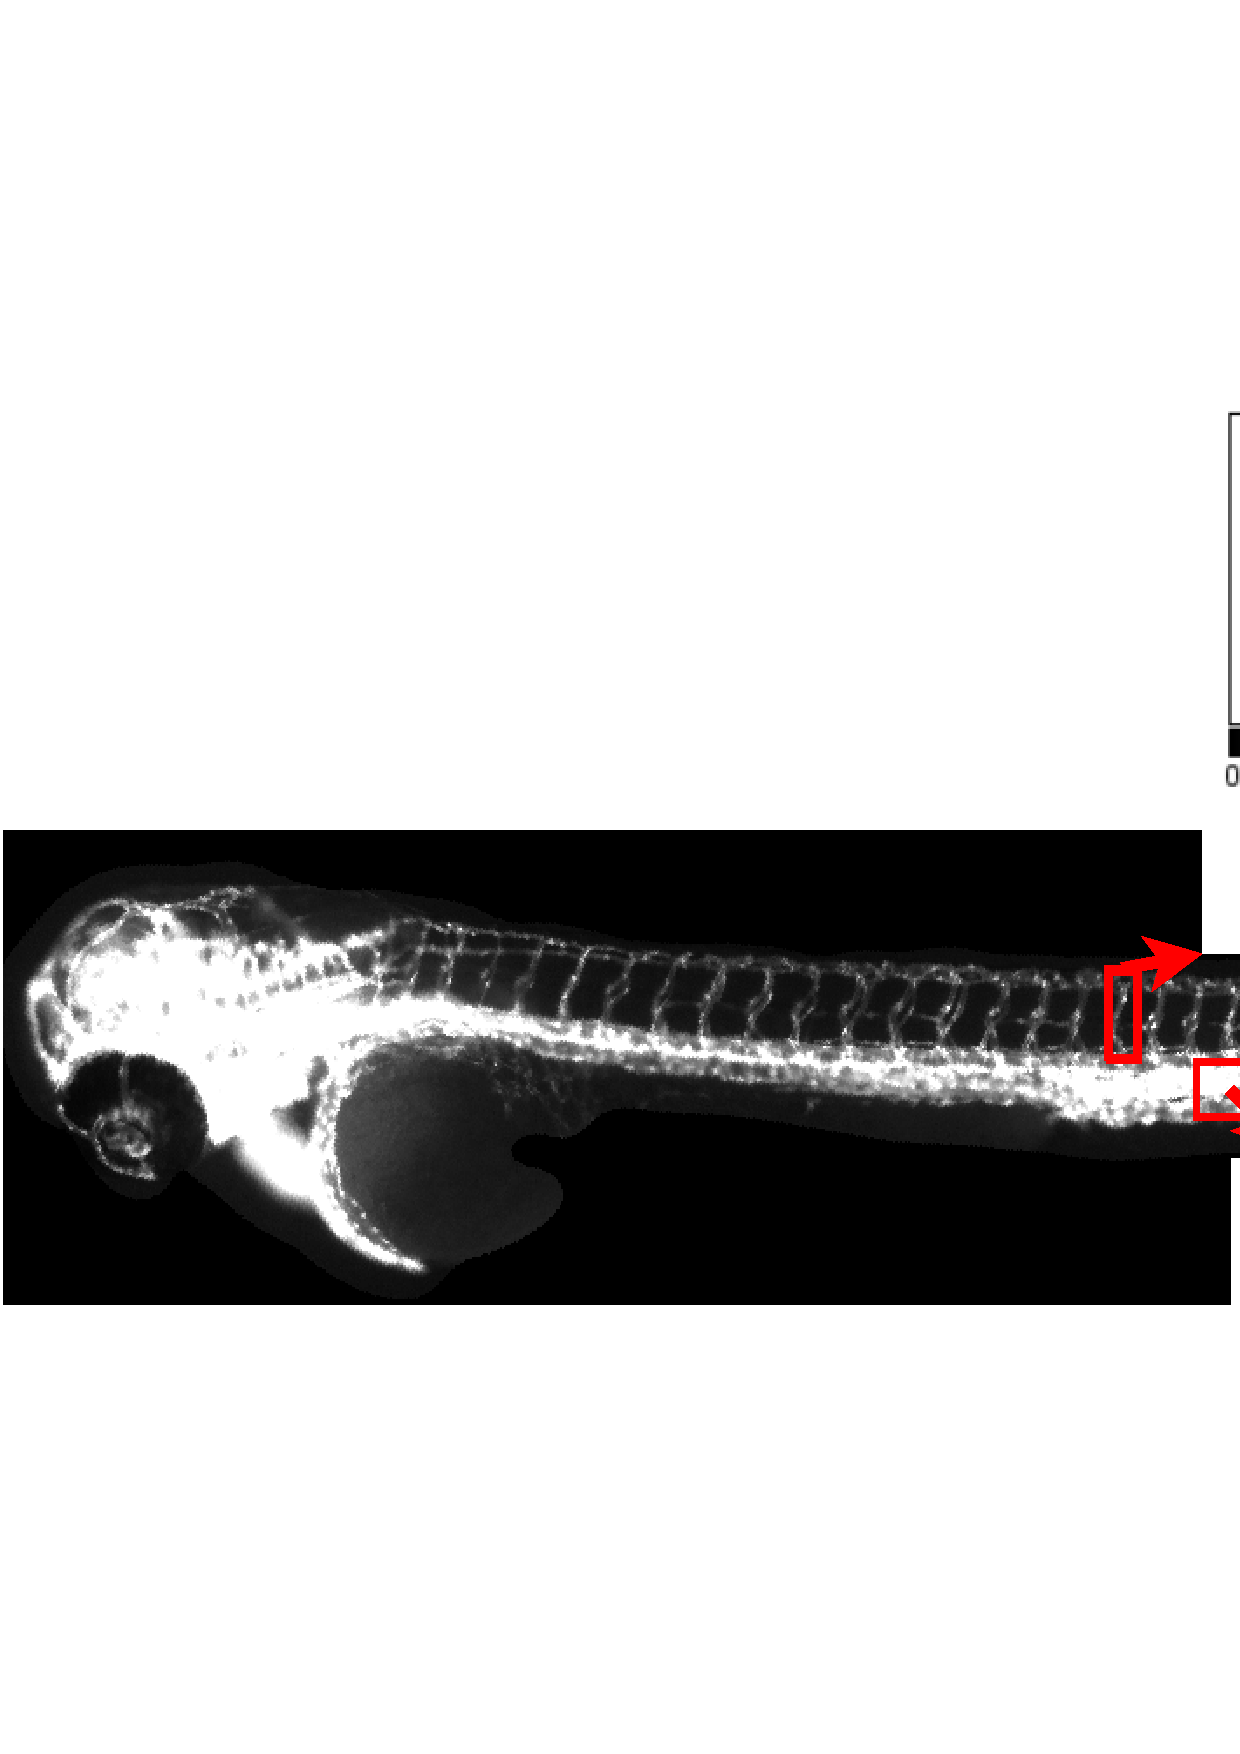
\includegraphics[scale=0.3]{figure/intensityProfile.png}
  \caption[Intensity profile of ISV + DLAV region compared to tail + head region]{The difference in intensity profile of ISV + DLAV region compared to tail + head region. The difference in intensity profile average value is more than 150.}
  \label{intensityProfile}
\end{figure}

We enhanced contrast, to further exemplify differences in their intensity value. Intermodes threshold based on bimodal distribution is well suited for separating ISV + DLAV from rest of embryo. The histogram is smoothed using a running average of size 3, until there are only two local maxima. The threshold value is the average of two peaks. 

\begin{figure}[htb] 
 \centering
    \includegraphics[scale=0.25]{figure/headYolkPosition.png}
  \caption[Procedure for finding head yolk position]{ Procedure for finding head yolk position. Figure \ref{noiseRem}B is obtained by masking out ISV + DLAV region from fig. \ref{noiseRem}A. Skeleton (fig. \ref{noiseRem}C) of mask is used to find the position of head and yolk and point of intersection of head and yolk region, and hence remove the rest of data.}
  \label{noiseRem}
\end{figure}

\begin{figure}[htb] 
\centering
    \includegraphics[scale=0.65]{figure/isvCvpRegion.png}  
  \caption[ROI Detection]{Procedure for extracting ISV + DLAV region and tail region. Figure \ref{region}D is obtained by masking segmented region shown in fig. \ref{region}b and removing head region. Figure \ref{region}E is obtained by masking out segmented region fig. \ref{region}B from \ref{region}A. Figure \ref{region}C is used to remove isolated region from head and yolk.}
  \label{region}
\end{figure}

Although above step separates zebrafish embryo into two region. But there is still some isolated portion of head, and yolk region left to be masked out. Specifically for tail + head region, we want to mask out only tail region. Skeleton of segmented image is used to find head, and yolk position. We can have two possibilities for head and yolk. Head can be on right side of image (fig. \ref{noiseRem}D) or left side of image. Yolk can face up or upside down (fig. \ref{noiseRem}D). We scan the skeleton image from top (from origin) along image width and store pixel values in pixelLocUp. Similarly, we scan the skeleton image from bottom (from height) along image width and store pixel values in pixelLocDown. Next we compute the euclidean distance between each pair of entries in pixelLocUp, and pixelLocDown as described in algorithm ~\ref{alg:cleanImage}. Next step is to find the position of yolk, if yolk is facing up or upside down (algorithm ~\ref{alg:yolkLocation}). Lastly for finding head location we use steps described in algorithm ~\ref{alg:headLocation}.

\begin{algorithm}
  \caption{Algorithm for finding distances between skeleton point from top and bottom.}
  \begin{algorithmic}
	\For  {$i=1$ to $height$} 
	\For  {$j=1$ to $width$} 
	\If {($Image(i,j) == 255$)}
			 \State  $pixelLocUp = [pixelLocUp; i j]$
			\State break
    \EndIf  
	\EndFor
	\EndFor
	\For  {$i=height$ to $1$} 
	\For  {$j=width$ to $1$} 
	\If {($Image(i,j) == 255$)}
			\State  $pixelLocDown = [pixelLocDown; i  j]$
			\State break
  \EndIf  
	\EndFor
	\EndFor
		
 \LineComment{pairwise Euclidean distance for pixelLocUp, pixelLocDown}
 \State pixelLocUpDist = dist(pixelLoUp, pixelLocUp)
 \State pixelLocDownDist = dist(pixelLocDown, pixelLocDown)
\end{algorithmic}
\label{alg:cleanImage}
\end{algorithm}

\begin{algorithm}
  \caption{Algorithm for finding yolk position, and cleaning region containing yolk }
  \begin{algorithmic}
 \LineComment{Yolk is facing up}
 \If {($max(pixelLocUpDist) > max(pixelLocDownDist)$)} 
    \State $top =  true$
    \State $location =  find(pixelLocUpDist == max(pixelLocDist))$
\LineComment{Yolk is facing down}
 \Else
   \State $top =  false$
   \State $location =  find(pixelLocDownDist == max(pixelLocDownDist))$
\EndIf 
\LineComment {clean image above pixelLocUp}
\If {( $top == true$ )}
	\For {$i = 1$ to $pixelLocUp.size$}
		\For {$j = 1$ to $pixelLocUp[i][1]$}
			\State $Image(j, pixelLocUp[i][2]) = 0$
		\EndFor
	\EndFor
\LineComment {clean image below pixelLocDown}
\Else
	\For {$i = 1$ to $pixelLocDown.size$}
		\For {$j = height$ to $pixelLocDown[i][1]$}
			\State $Image(j, pixelLocDown[i][2]) = 0$
		\EndFor
	\EndFor
\EndIf
\end{algorithmic}
\label{alg:yolkLocation}
\end{algorithm}

\begin{algorithm}
  \caption{Algorithm for finding head position and clean image containing head region}
  \begin{algorithmic}
\LineComment {head is on right side}
\If {($dist( location, 0) > dist(location, width)$)}
	\For {$i = 1$ to $height$}
		\For {$j = location.y$ to $width$}
		\LineComment {clean image from head location to width}
			\State $Image(i,j) = 0$
		\EndFor
		\EndFor	
\LineComment {head is on left side}
\Else 
	\For {$i = 1$ to $location.x$}
		\For {$j = 1$ to $location.y$}
	\LineComment {clean image from origin to head location}
			\State $Image(i,j) = 0$
	 \EndFor
	\EndFor
\EndIf
\end{algorithmic}
\label{alg:headLocation}
\end{algorithm}

After eliminating yolk and head region, we are confined with two ROI, one enclosing ISV and other enclosing tail (fig. \ref{region}E, \ref{region}D).

\section{Intersegmental Vessel Segmentation}\label{sec:isvseg}

Next we need to extract ISV from image. Extraction of ISV is challenging since it varies in size, local contrast is unstable, high curvature, and noisy. The ability to segment and quantify vessels, especially with smaller diameter, is limited by noise and contrast. 


\subsection{Eigen Analysis}

The eigenanalysis of Hessian matrix is a crucial method for vessel detection. Hessian matrix components approximate 2nd order derivatives, and hence represents the shape information in terms of both, quality and quantity. Particularly interesting are the eigenvalues and eigenvectors of Hessian matrix. In this work, we are presenting the ISV detection method based on eigenanalysis of image Hessian matrix combined with multiscale image analysis. A segmentation method incorporating vessel direction and the eigenvector of the Hessian matrix is used for vessel detection and to obtain a segmented vessel tree.

The common approach to analyze local shape of a $2D$ image I is to consider its Taylor Expansion in the neighborhood of a point $x_{0}$. 

\begin{equation}
I(x + x_{0}) \approx I(x_{0}) + \Delta x^{T} \nabla I(x_{0}) + \Delta x^{T} \nabla H(x_{0}) \Delta (x)
\end{equation}

where $\nabla$I is the gradient vector and H denote Hessian matrix of second-order partial derivatives of an image I.

\begin{equation}
H = \begin{bmatrix}
\frac{\partial^2 I}{\partial x^2}&\frac{\partial^2 I}{\partial x \partial y}\\ \frac{\partial^2 I}{\partial y \partial x}&\frac{\partial^2 I}{\partial y^2}
\end{bmatrix}
\end{equation}

For a given pixel of an image a Hessian matrix is composed of second order partial derivatives. Second order derivatives locally approximates the structure of an image. To solve these differential operators in a well-posed fashion we use concepts of linear scale space theory \cite{Koenderink84}. In this framework differentiation is defined as a convolution with derivatives of Gaussian:
\begin{equation}
\frac{\partial I}{\partial x} = I(x) * \frac{\partial G(x,\sigma)}{\partial x}
\end{equation}

where the Gaussian is defined as:

\begin{equation}
G(x,\sigma) = \frac{1}{\sqrt{2\pi\sigma^2}} \exp(-\frac{x}{2\sigma^2})
\end{equation}

where the parameter $\sigma$ is the standard deviation of the Gaussian kernel, it controls the scale and the smoothing. With increasing the scale the image gets less detailed. The scale allows to search for objects of similar dimensions as  the chosen scale. Let the eigenvalues of the Hessian matrix be $\lambda_{1}$ and $\lambda_{2}$ $(\lambda_{1} \geq \lambda_{2})$ and corresponding eigenvectors be $v_{1}$ and $v_{2}$. The eigenvalues $\lambda_{1}$ and $\lambda_{2}$ of the Hessian matrix can be calculated through the following equation:

\begin{equation}
\Delta (H - I*\lambda) = 0
\end{equation}

where I is an identity matrix and $\lambda$ is set of eigenvalues.

The eigenvalue of Hessian matrix are called principal curvature. The eigenvalues of the Hessian matrix evaluated at a point encodes the local morphology in all direction in terms of curvature \cite{Descoteaux05}. The highest eigenvalue $\lambda_{1}$ corresponds to maximum change in curvature, and corresponding eigenvector gives a direction of maximum change \cite{Frangi98multiscalevessel}. The eigenvector $v_{2}$ is orthogonal to the vector $v_{1}$.  

Since vessels appear in different sizes it is important to introduce a measurement scale which varies within a certain range, which matches the local feature size. Evaluating the eigenvalue in a scale-space shows local morphology change with scale. The scale-space theory introduced by Lindeberg \cite{Lindeberg96} uses for the purpose of detail removal a convolution with a Gaussian kernel. We denote the eigenvectors of the Hessian, $H(x,\sigma)$, at sampling location x and scale $\sigma$ as $v_{1}(x,\sigma), v_{2}(x,\sigma)$. The eigenvalues are denoted by $\lambda_{1}(x,\sigma),\lambda_{2}(x,\sigma)$.

ISVs are extracted by tracing the direction of maximum eigenvalue normal to x-axis. Our response function is calculated from eigenvalue evaluated by extracting the direction of maximum eigenvalue. For each location, we compute the angle between eigenvector corresponding to maximum eigenvalue and vector X in x (horizontal) direction. 

\begin{equation}
h(v_{1}(x,\sigma), X) = \frac{v_{1}(x,\sigma) \cdot X}{\|v_{1}(x,\sigma)\|\|X\|}
\end{equation}

We analyze the response from each scale within pre-determined range, and select the maximum eigenvalue based on $h$. Since ISV in images exists with varying size, it is logical to perform feature extraction at the scale which matches the ISV size. The strongest response (with respect to $\sigma$) over scales directly corresponds with width of object \cite{Lindeberg96}. For this purpose, our parameter selection is based on prior measurement of width of objects. From our data set, we manually measure the width of ISV. We randomly select $\frac{1}{15}$ images from our dataset, and measure the width of vessel, and use the range of values for scale parameter. From our observation, we found radius of ISV to be in range $[0.5, 3]$.

\begin{equation}\label{eq:isv}
r(x) = \begin{cases} \max_{\sigma} \lambda_{1}(x,\sigma) &\mbox{if } \beta \leq\ h(x, \sigma) \geq \alpha\\ 
0 & \mbox{if } otherwise \end{cases} 
\end{equation}
 
All pixels which satisfy \eqref{eq:isv} belongs to ISV. Parameter $\alpha$ is chosen to be $45$ and $\beta$ is chosen to be $135$. We want to remove all the pixels which are parallel or approximately parallel to horizontal axis. For our purposes, tolerance of $\pm45$ works well. We binarize ISV (say $b_{r}$) based on value from proposed adaptive Niblack thresholding.


\subsection{Adaptive Niblack thresholding}

Original Niblack's algorithm \cite{niblack1985} is a local thresholding method based on the calculation of the local mean and of local standard deviation. The threshold is calculated by the formula:

\begin{equation}\label{eq:niblack}
T = m + k*s
\end{equation}

where, m and s are the local mean and standard deviation of pixel values in local neighborhood, respectively. The size of the
neighborhood should be small enough to preserve local details, but at the same time large enough to suppress noise. k is the correction factor to adjust how much of the total object boundary is taken as a part of given object.
 
Instead of having fixed k, we use scale parameter which matches the ISV size. We can derive scale information from equation \eqref{eq:isv}. We return for every pixel the value of the scale (sigma) with the maximum eigenvalue from \eqref{eq:isv}. We utilized window size of $[125, 25]$ approximately based on box enclosing ISV.  
% output pixel value
 


\subsection{Linking vessels}

\begin{figure}[htb]
  \begin{center}
    \includegraphics[scale=0.25]{figure/highResponse.png}
  \end{center}
  \caption[ISV principal direction estimation]{Figure \ref{responseAnalysis}A is used in place of original image to depict the structure similar to of ISV. \ref{responseAnalysis}A shows the response of maximum eigenvalue corresponding to scale = 1 for principal direction. In top right fig. \ref{responseAnalysis}C, shows few isolated regions from DLAV. These regions are outliers and will be removed. Figure \ref{responseAnalysis}D perfectly captures the response corresponding to principal direction. Figure \ref{responseAnalysis}E shows the region whose principal direction is lies outside the $[\alpha, \beta]$, hence no response is generated. These regions are merged.}
  \label{responseAnalysis}
\end{figure}

Some ISV might appear disconnected, or some isolated response from DLAV region might be outliers as shown in fig. \ref{responseAnalysis}C. This happens when region along center of ISV, appears parallel to x-axis i.e. the angle of principal direction with horizontal axis does not fall in $[\alpha, \beta]$ as depicted in fig. \ref{responseAnalysis}E. We connect the disjoint ISV's and remove outlier from DLAV based on the feature set extracted form each ISV region. 

The broken ISV when region along center of ISV, appears parallel to x-axis i.e. the angle of principal direction with horizontal axis does not fall in $[\alpha, \beta]$ as depicted in fig. \ref{responseAnalysis}E. Here we use morphological operation to link the broken vessels segmented. We compute the maximum response from all vessels using \eqref{eq:isv}. We binarize $r_{a}(x)$ based on value from Adaptive Niblack thresholding and call it $b_{r_a}$. Parameter k is the value of the scale (sigma) with the maximum eigenvalue from \eqref{eq:all}.

\begin{equation}\label{eq:all}
r_{a}(x) = \max_{\sigma} \lambda_{1}(x,\sigma) 
\end{equation}

At each potential vessel pixel from $b_{r}$, we apply morphological closing using linear structure. The direction of the linear structure is perpendicular to the x-axis direction. We set the length of the linear structure as 10 pixels in the experiments. We retain all those potential vessel pixel from $b_{r}$ that belongs to $b_{r_a}$.

\subsection{Post Processing}

There are some isolated response from DLAV region which are outliers as shown in fig. \ref{responseAnalysis}C. We follow similar approach as for linking vessels, but instead we work with maximum response from vessels from DLAV region \eqref{eq:dlav}. We binarize $r_{d}(x)$ based on value from Niblack thresholding and call it $b_{r_d}$. Parameter k is the value of the scale(sigma) with the maximum eigenvalue from \eqref{eq:dlav}.

\begin{equation}\label{eq:dlav}
r_{d}(x) = \begin{cases} \max_{\sigma} \lambda_{1}(x,\sigma) &\mbox{if } \alpha < \ h(x, \sigma) > \beta\\ 
0 & \mbox{if } otherwise \end{cases} 
\end{equation}

At each potential vessel pixel from $b_{r_d}$, we apply morphological closing using linear structure. The direction of the linear structure is parallel to the x-axis direction. We set the length of the linear structure as 10 pixels in the experiments. We remove all those potential vessel pixel from $b_{r}$ that belongs to $b_{r_d}$.


\section{Caudal Vein Plexus Segmentation}

After extracting ROI enclosing CVP as shown in fig. \ref{region}d. We use structural properties of CVP for segmentation. 

\begin{figure}[htb] \centering
\includegraphics[scale = 0.55]{figure/cvpSeg.png}
	 \caption[CVP Segmentation]{Procedure for CVP segmentation. Figure \ref{seg}A is a region enclosing CVP. Curve $C$ in blue represents lower boundary of tail region along midpoint of tail. Figure \ref{seg}B $C$ is smoothed using moving average filter. Pink points represents local maxima and green points represents local minima. Circled point represents the CVP region start location. CVP start position is the mid point of the local curve with largest steepness. Figure \ref{seg}C is the segmented CVP obtained by masking out segmented region from fig. \ref{noiseRem}A with fig. \ref{seg}A from start location of CVP.}
 \label{seg}
\end{figure}

The intuition behind our method is that there is a high gradient associated with transition of PCV region to CVP region in zebrafish. For this purpose, we trace the curve $C$ along mid point $m$ of lower boundary of the tail.Lets $C$  be represented as:

					 \begin{equation}
						C =  ((x_{i}, y_{i}), i= 1,2,\ldots, n)						
						\end{equation} 
						
We compute the slope of the cure as: 

				\begin{equation}
				S =  (\frac{dy_{i}}{dx_{i}}, i= 1,2,\ldots, n)
				\end{equation} 
				
S is smoothed using moving average filter. Let H and L denote the set of local maxima and local minima along S. Let v = $(h_{i0}, l_{j0})$ denote local maxima and local minima, respectively, such that:

					  \begin{align*}
						\bmod(h_{i0} - l_{j0}) \geq \bmod(h_{i} - l_{j}), 
						    \forall h_{i} \in H, \forall l_{j} \in L,  j-1 \leq i \leq j
						\end{align*}  
						
Point $p$ where the CVP starts is given by:

				\begin{equation}\label{eq:cvp}
				p = \begin{cases} \frac{h_{i0} + l_{j0}}{2} & \mbox{if } H \neq \emptyset, L \neq \emptyset\\ 
				m &  otherwise \end{cases} 
				\end{equation}  
				\normalsize
				
$p$ signifies the mid point along the curve with maximum change in slope. CVP is obtained by masking region shown in fig. \ref{noiseRem}A from segmented region shown in fig. \ref{seg}C from start location $p$ of CVP.